\section{Design}

\subsection{The Visual Language}
\begin{frame}[allowframebreaks]{The Visual Language}
\begin{itemize}
    \vspace{-0.5cm}
    \item The analysis of \moise{} and the creation of a focus group brought to the following design
    \vspace{0.5cm}
    \item Building blocks of the organization's \textbf{structure}:
\end{itemize}

\begin{columns}
    \begin{column}{0.5\textwidth}
        \begin{figure}
            \centering
            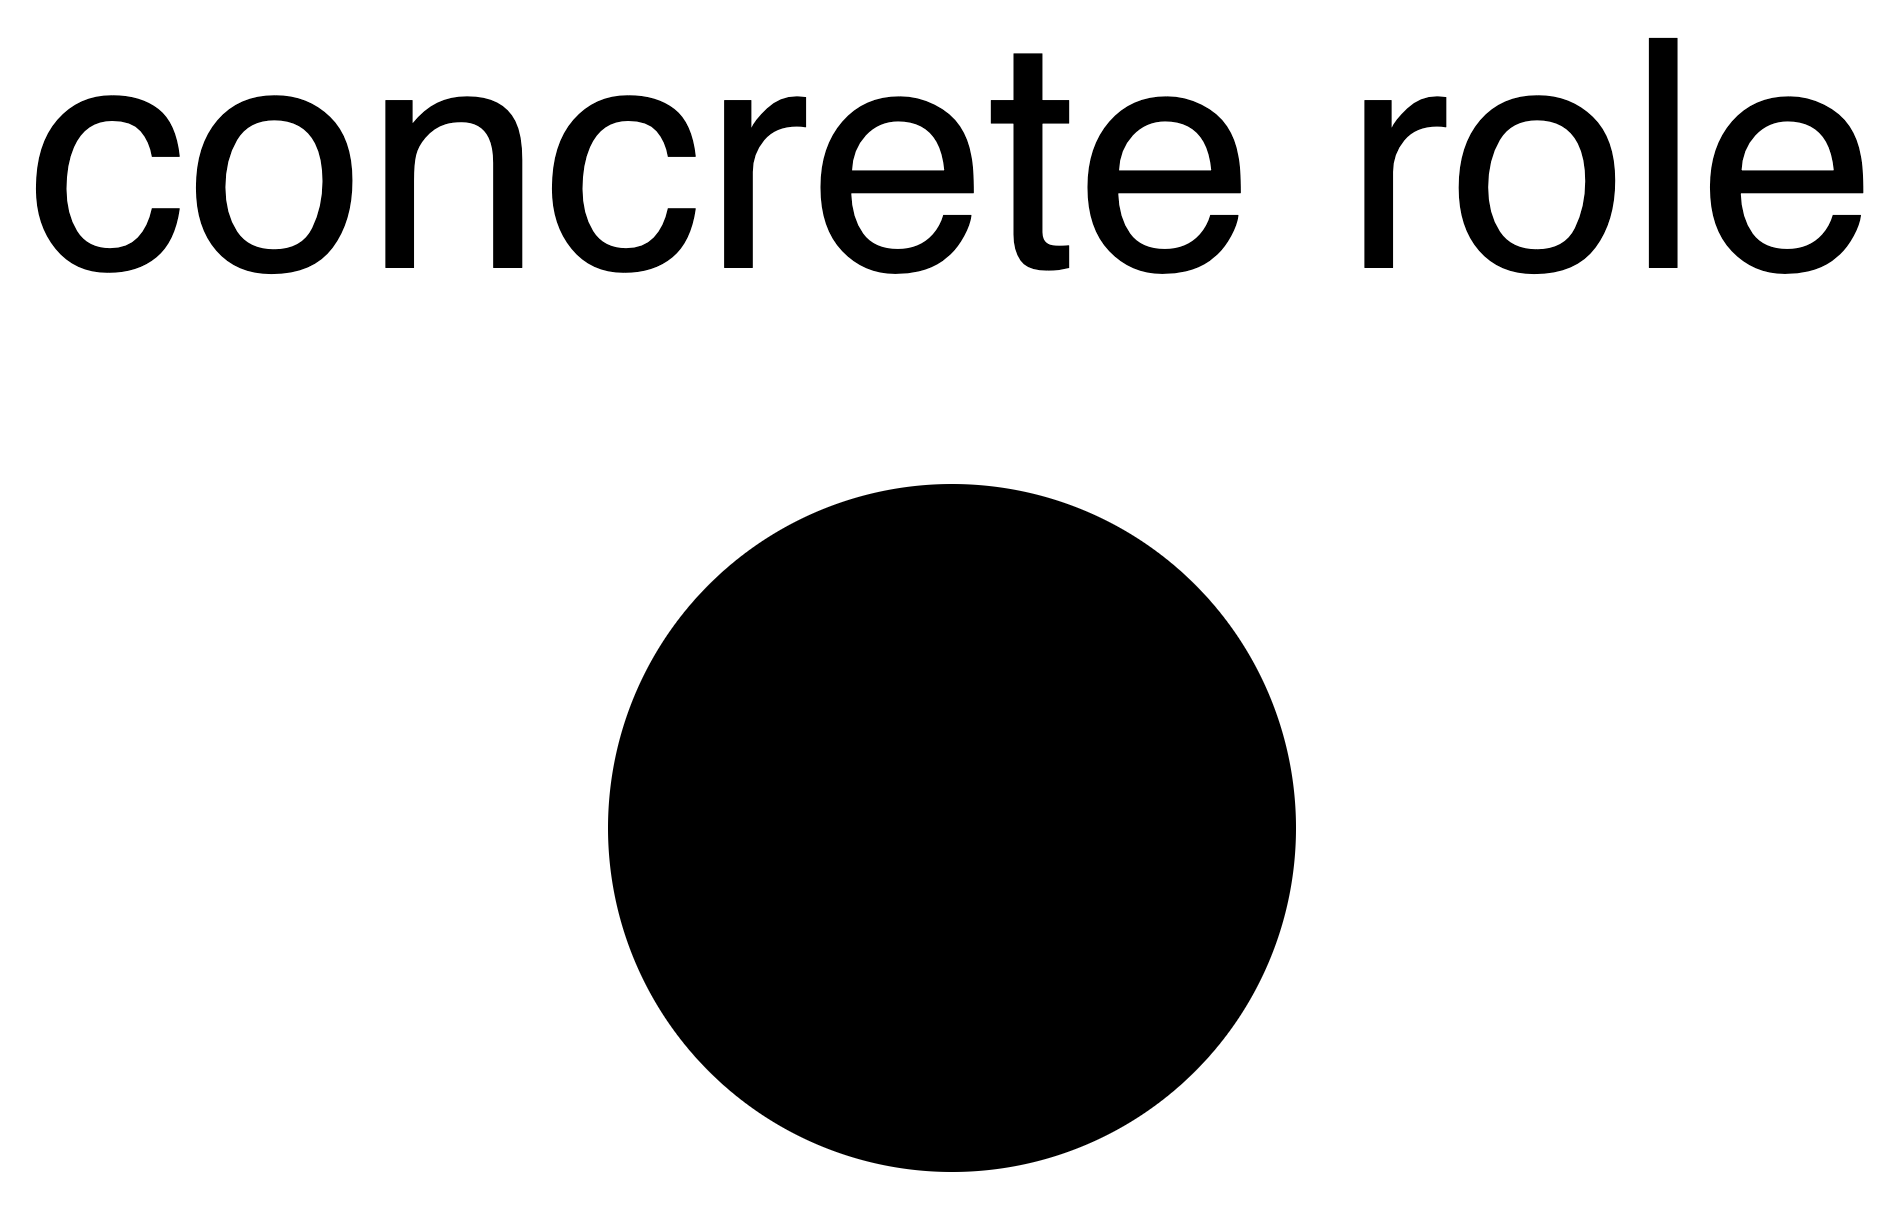
\includegraphics[width=0.35\textwidth]{images/visual-language/concrete-role.png}
        \end{figure}
    \end{column}
    \begin{column}{0.5\textwidth}
        \begin{figure}
            \centering
            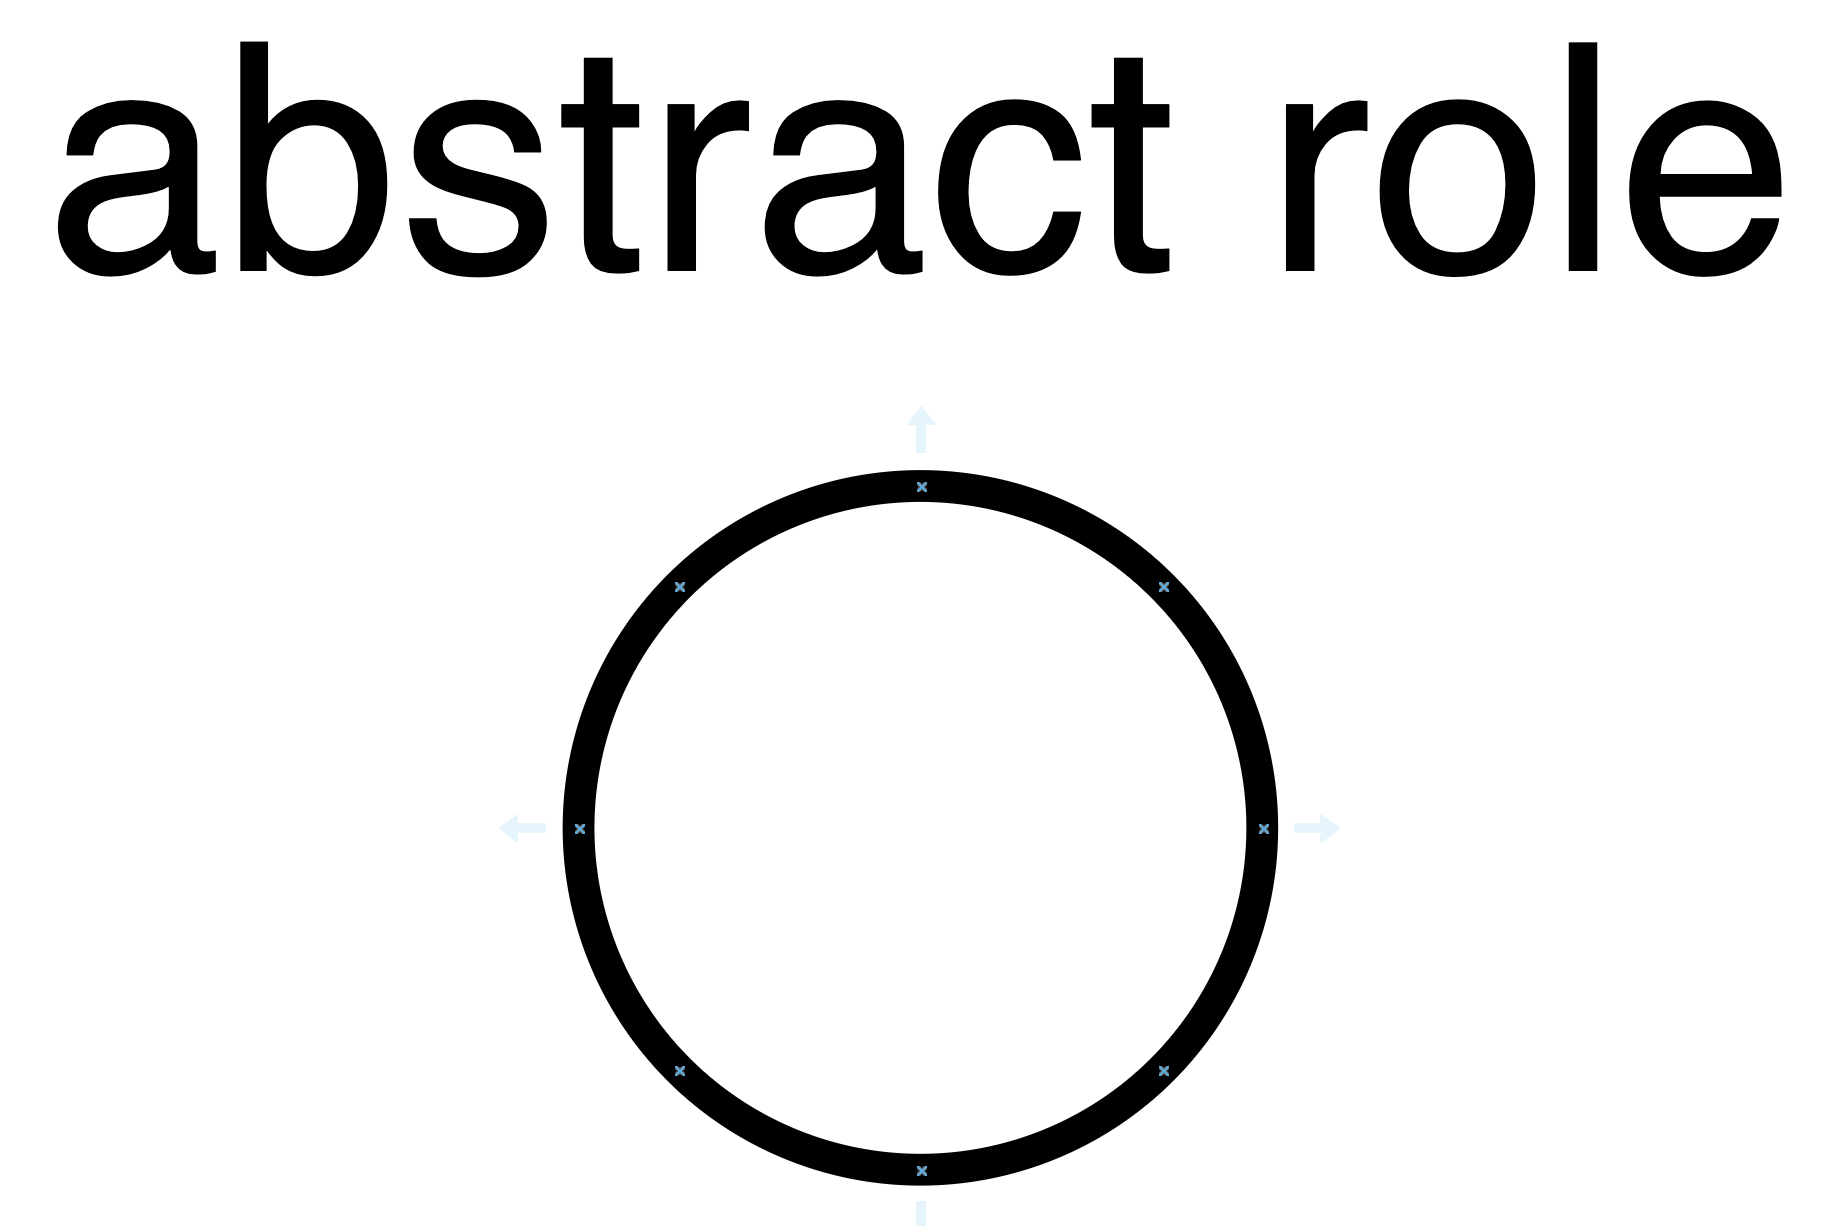
\includegraphics[width=0.35\textwidth]{images/visual-language/abstract-role.png}
        \end{figure}
    \end{column}
\end{columns}

\begin{columns}
    \begin{column}{0.5\textwidth}
        \begin{figure}
            \centering
            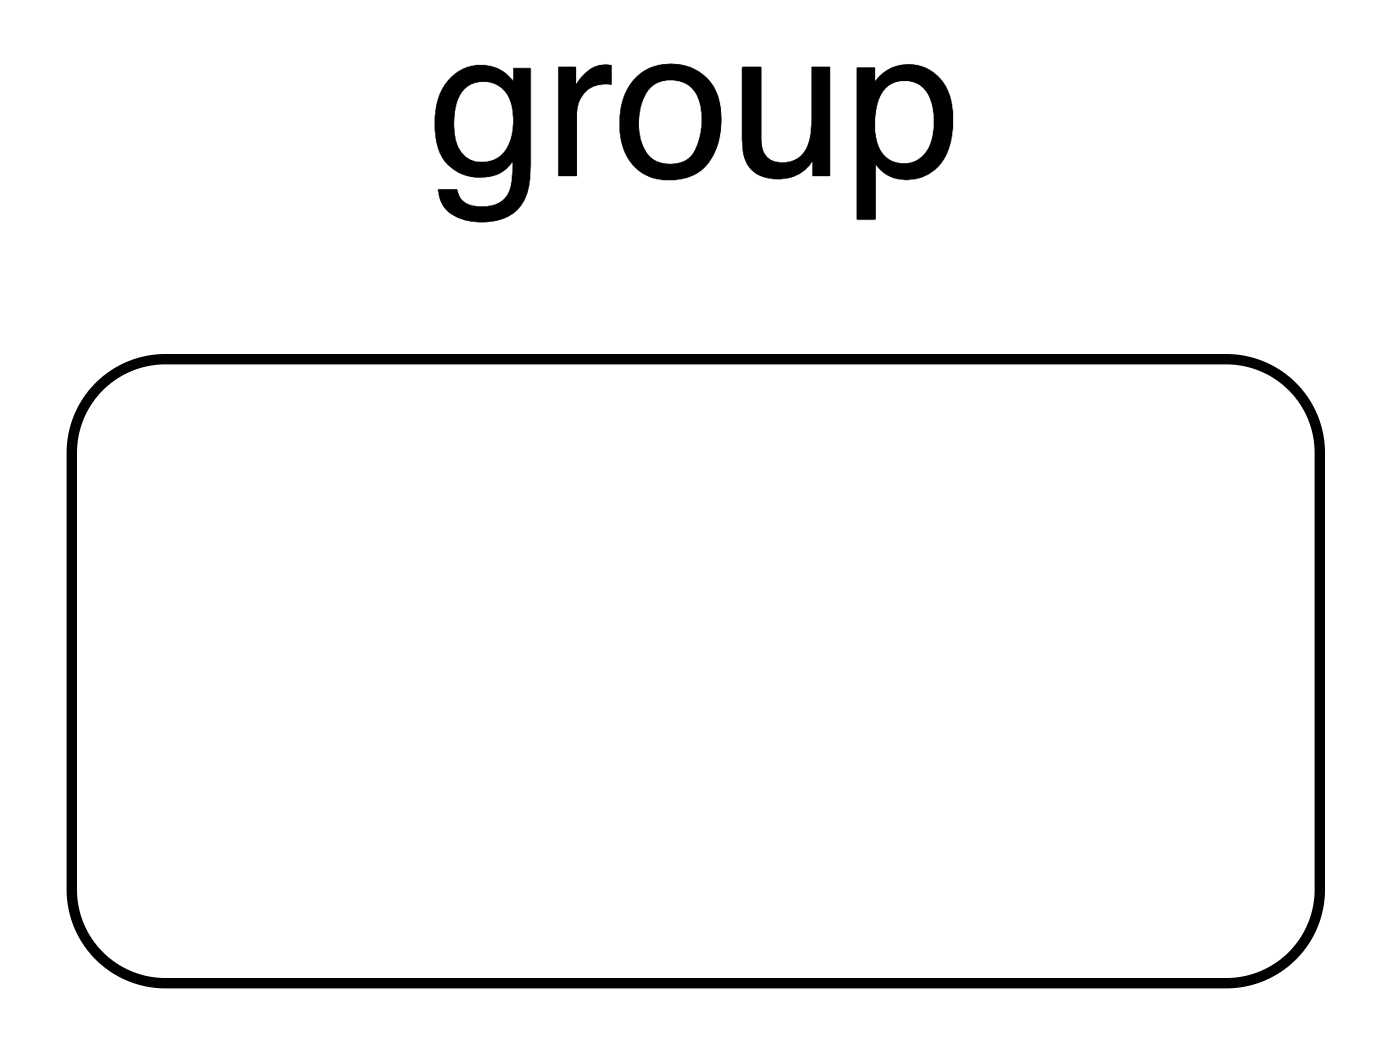
\includegraphics[width=0.35\textwidth]{images/visual-language/group.png}
        \end{figure}
    \end{column}
    \begin{column}{0.25\textwidth}
        \begin{figure}
            \centering
            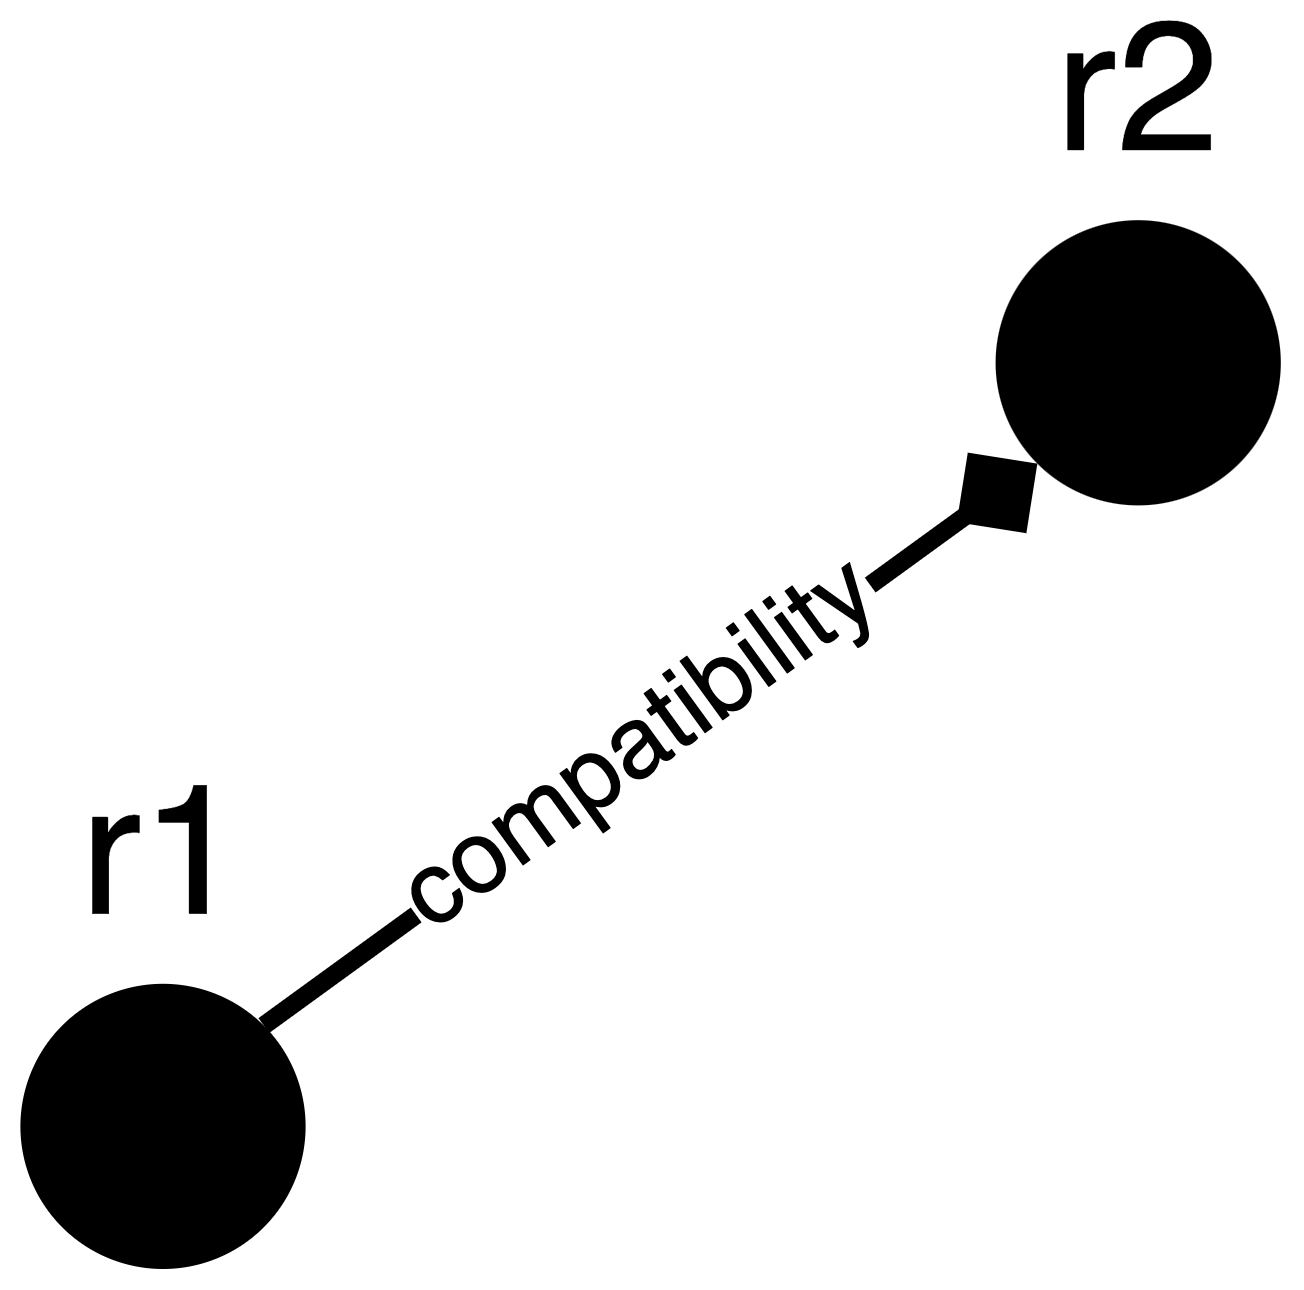
\includegraphics[width=0.7\textwidth]{images/visual-language/compatibility.png}
        \end{figure}
    \end{column}
    \begin{column}{0.25\textwidth}
        \begin{figure}
            \centering
            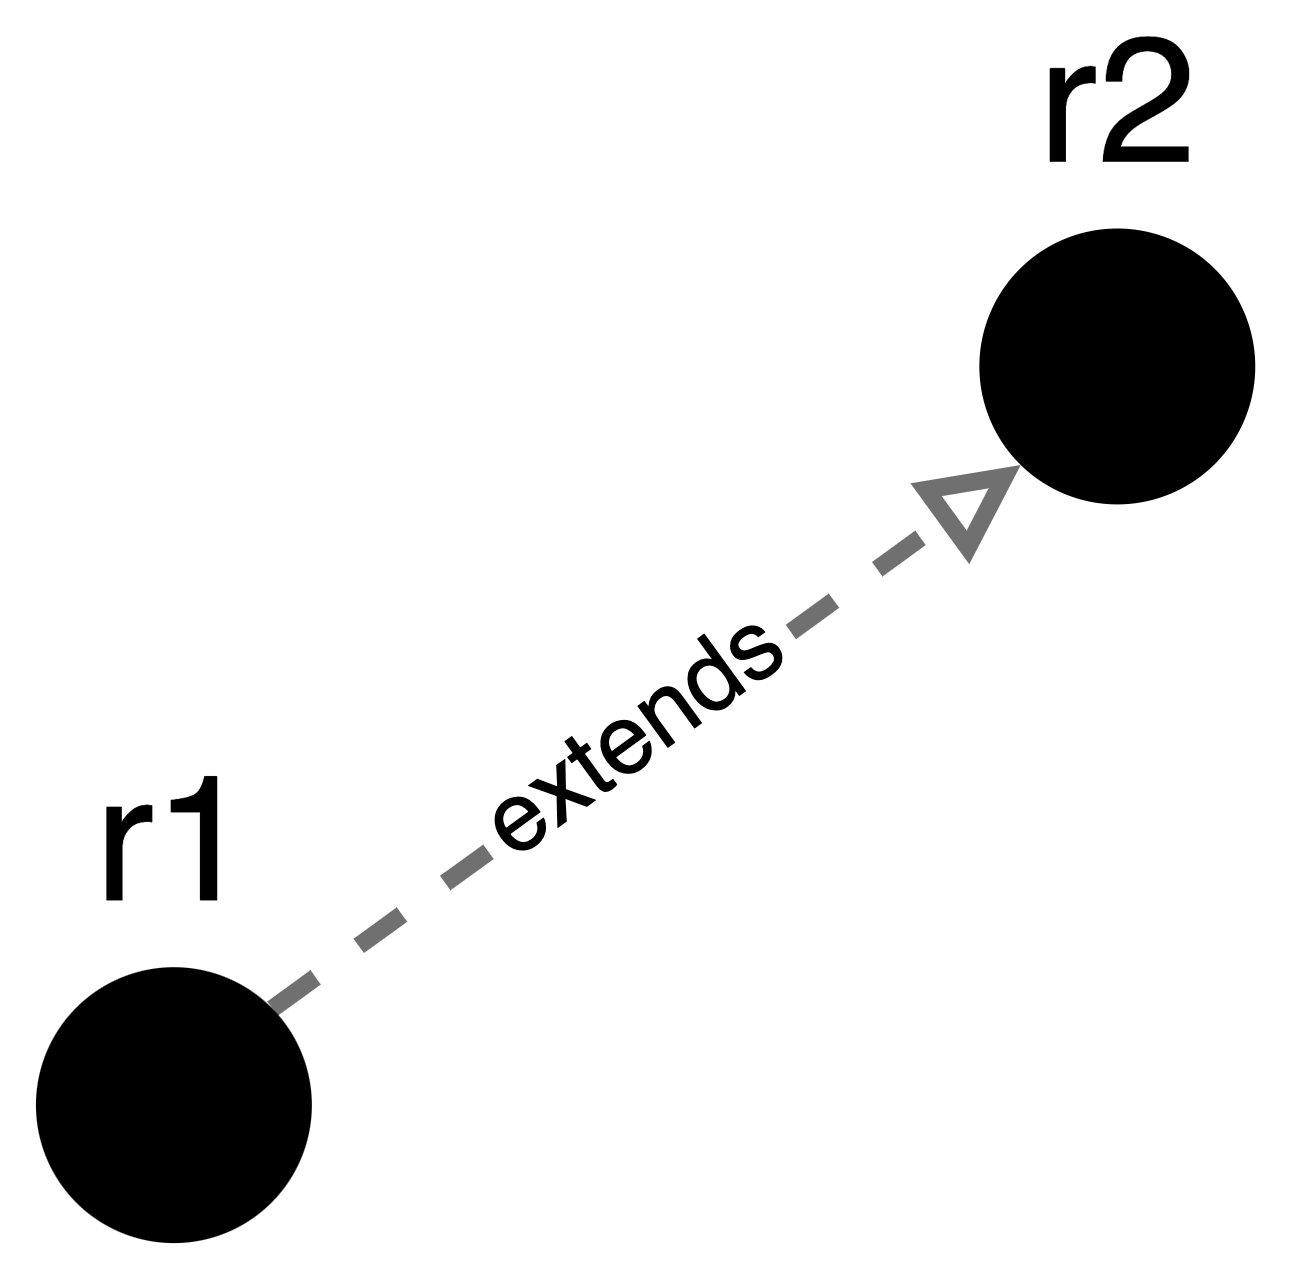
\includegraphics[width=0.7\textwidth]{images/visual-language/extension.png}
        \end{figure}
    \end{column}
\end{columns}

\framebreak

\begin{itemize}
    \vspace{-0.5cm}
    \item The analysis of \moise{} and the creation of a focus group brought to the following design
    \vspace{0.5cm}
    \item Building blocks of the organization's \textbf{behavior}:
\end{itemize}

\begin{columns}
    \begin{column}{0.5\textwidth}
        \begin{figure}
            \centering
            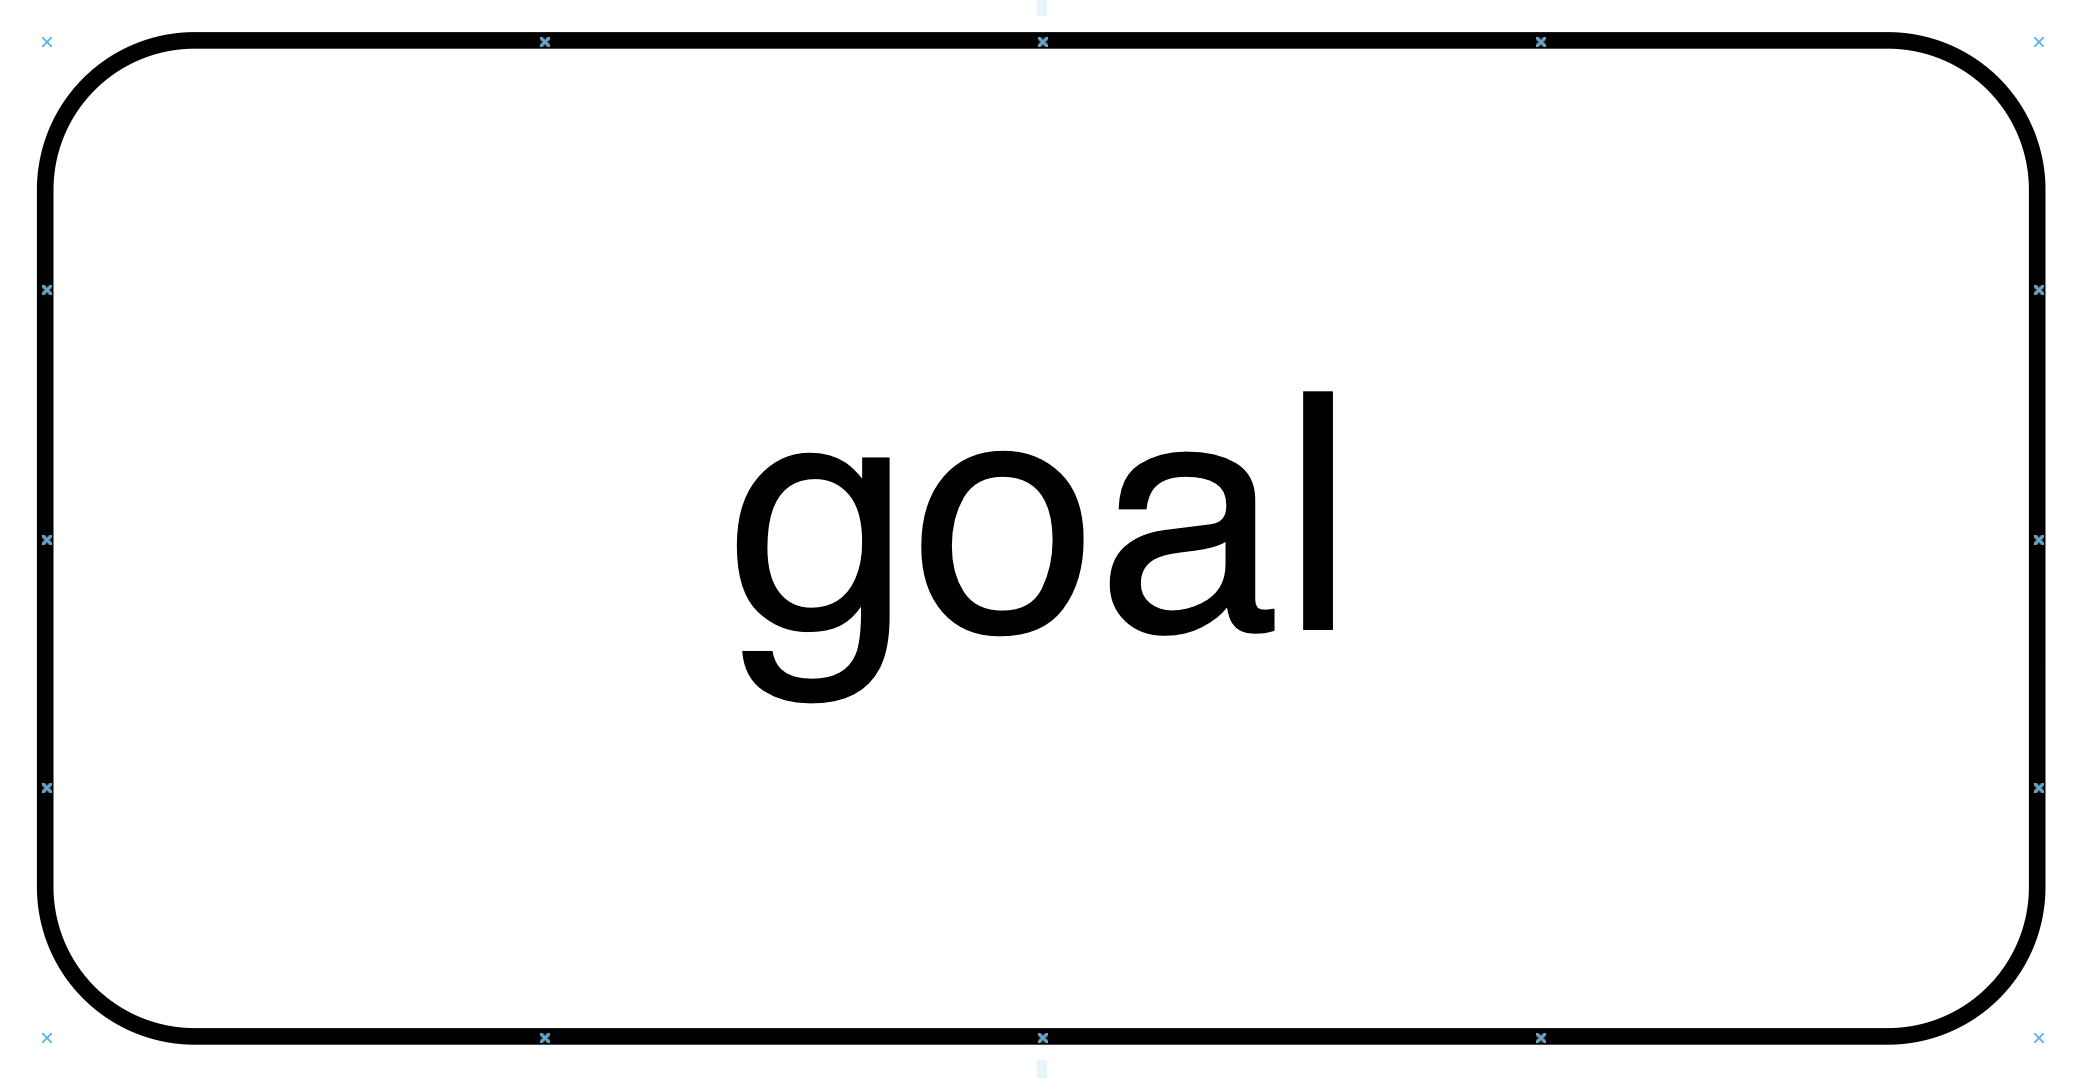
\includegraphics[width=0.35\textwidth]{images/visual-language/goal.png}
        \end{figure}
    \end{column}
    \begin{column}{0.5\textwidth}
        \begin{figure}
            \centering
            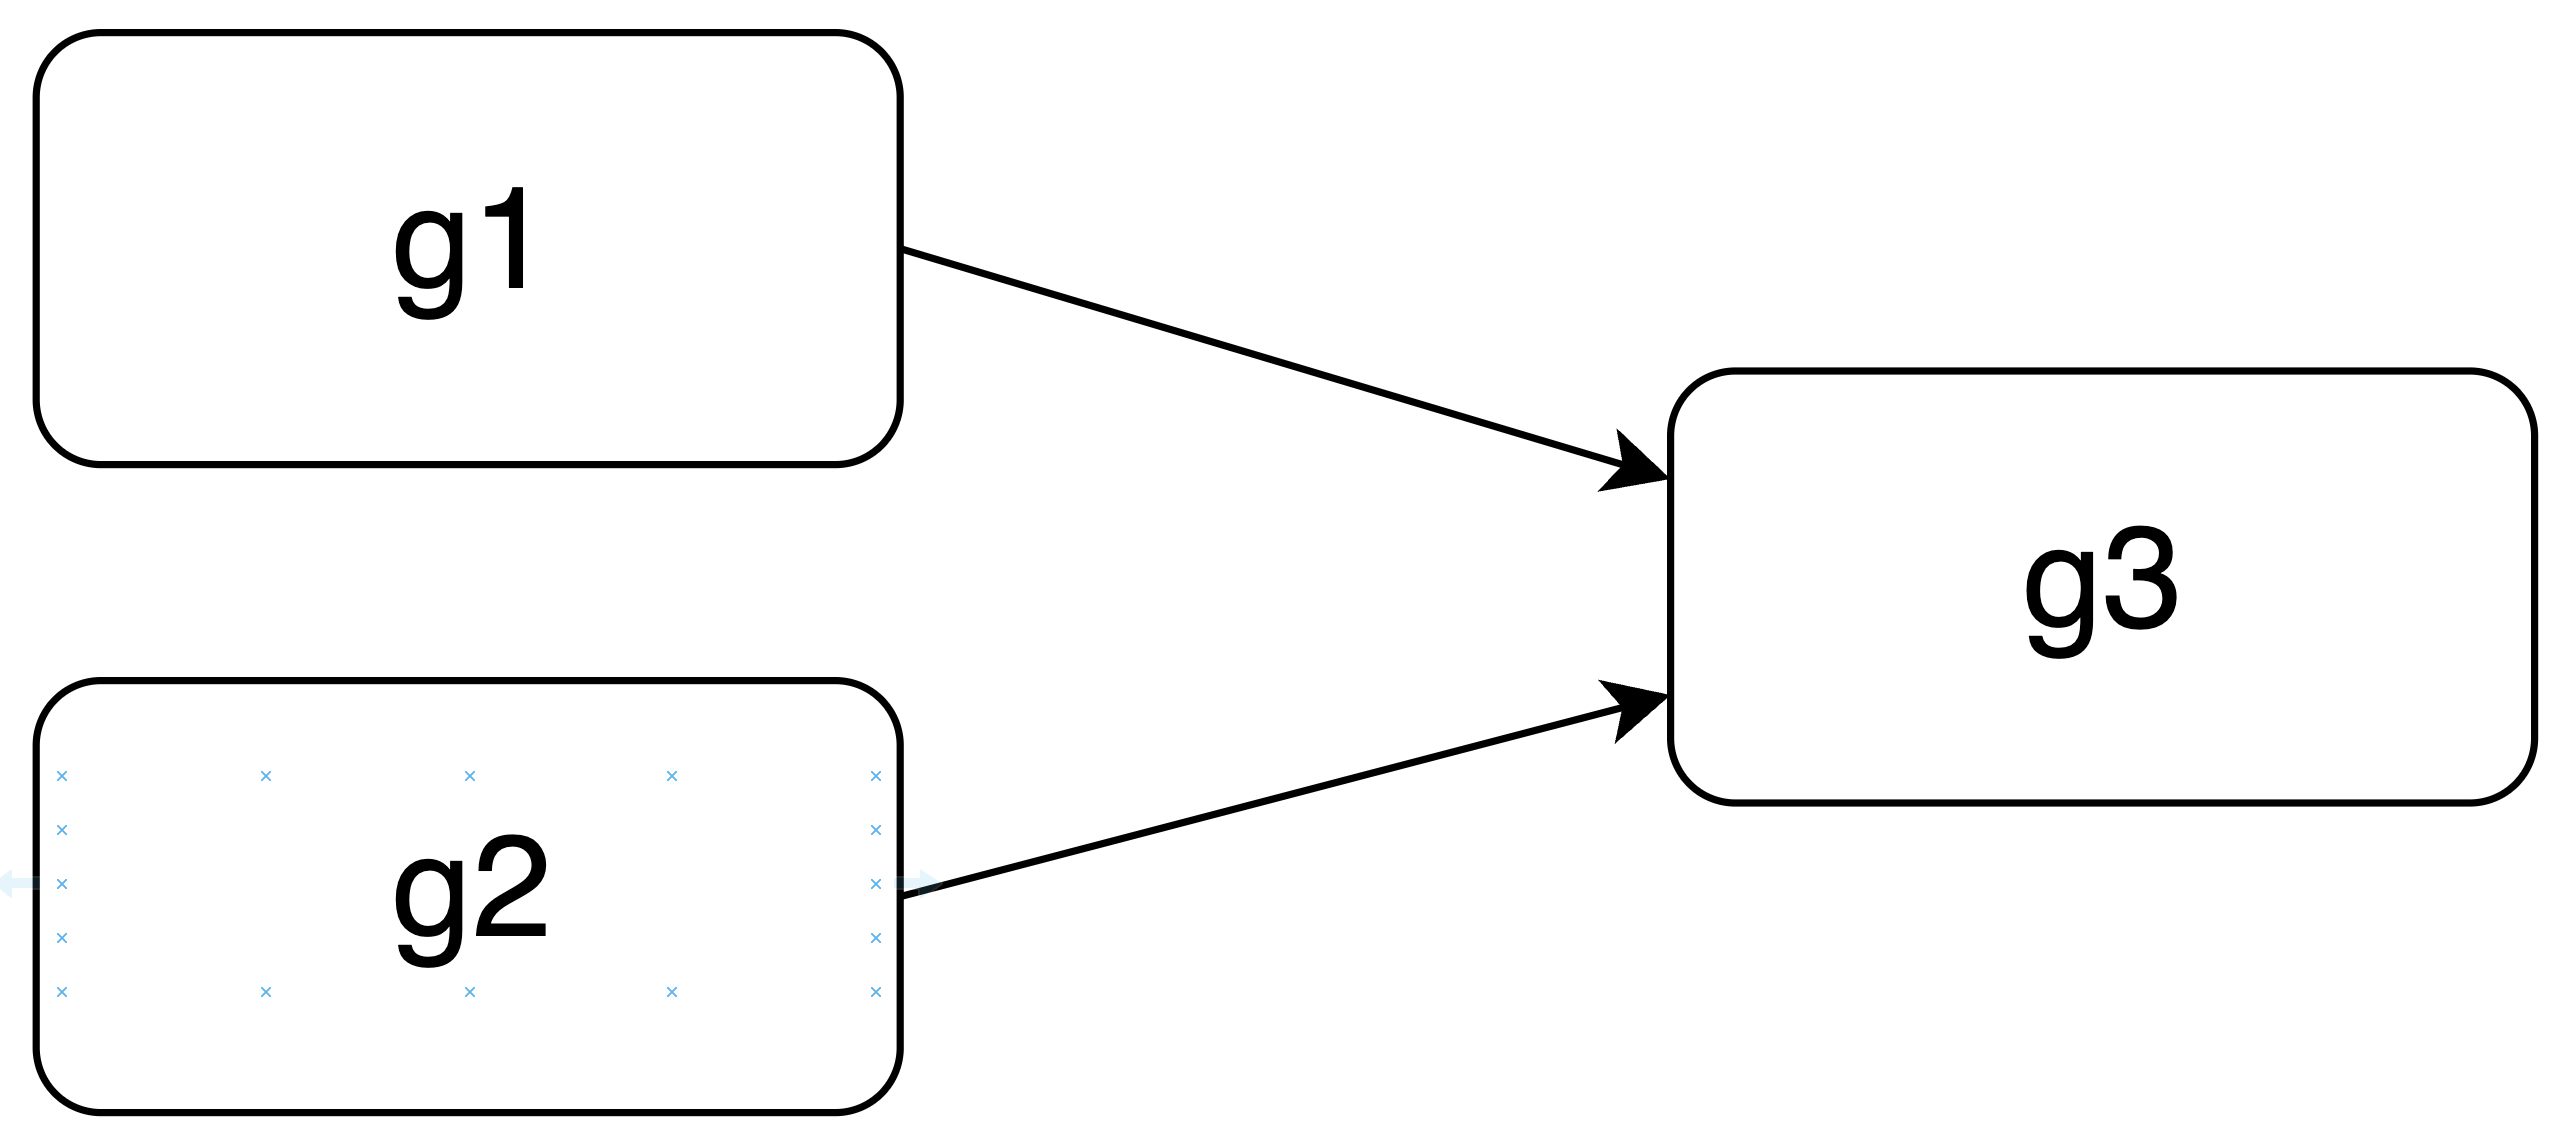
\includegraphics[width=0.7\textwidth]{images/visual-language/dependency-and.png}
        \end{figure}
    \end{column}
\end{columns}

\begin{columns}
    \begin{column}{0.5\textwidth}
        \begin{figure}
            \centering
            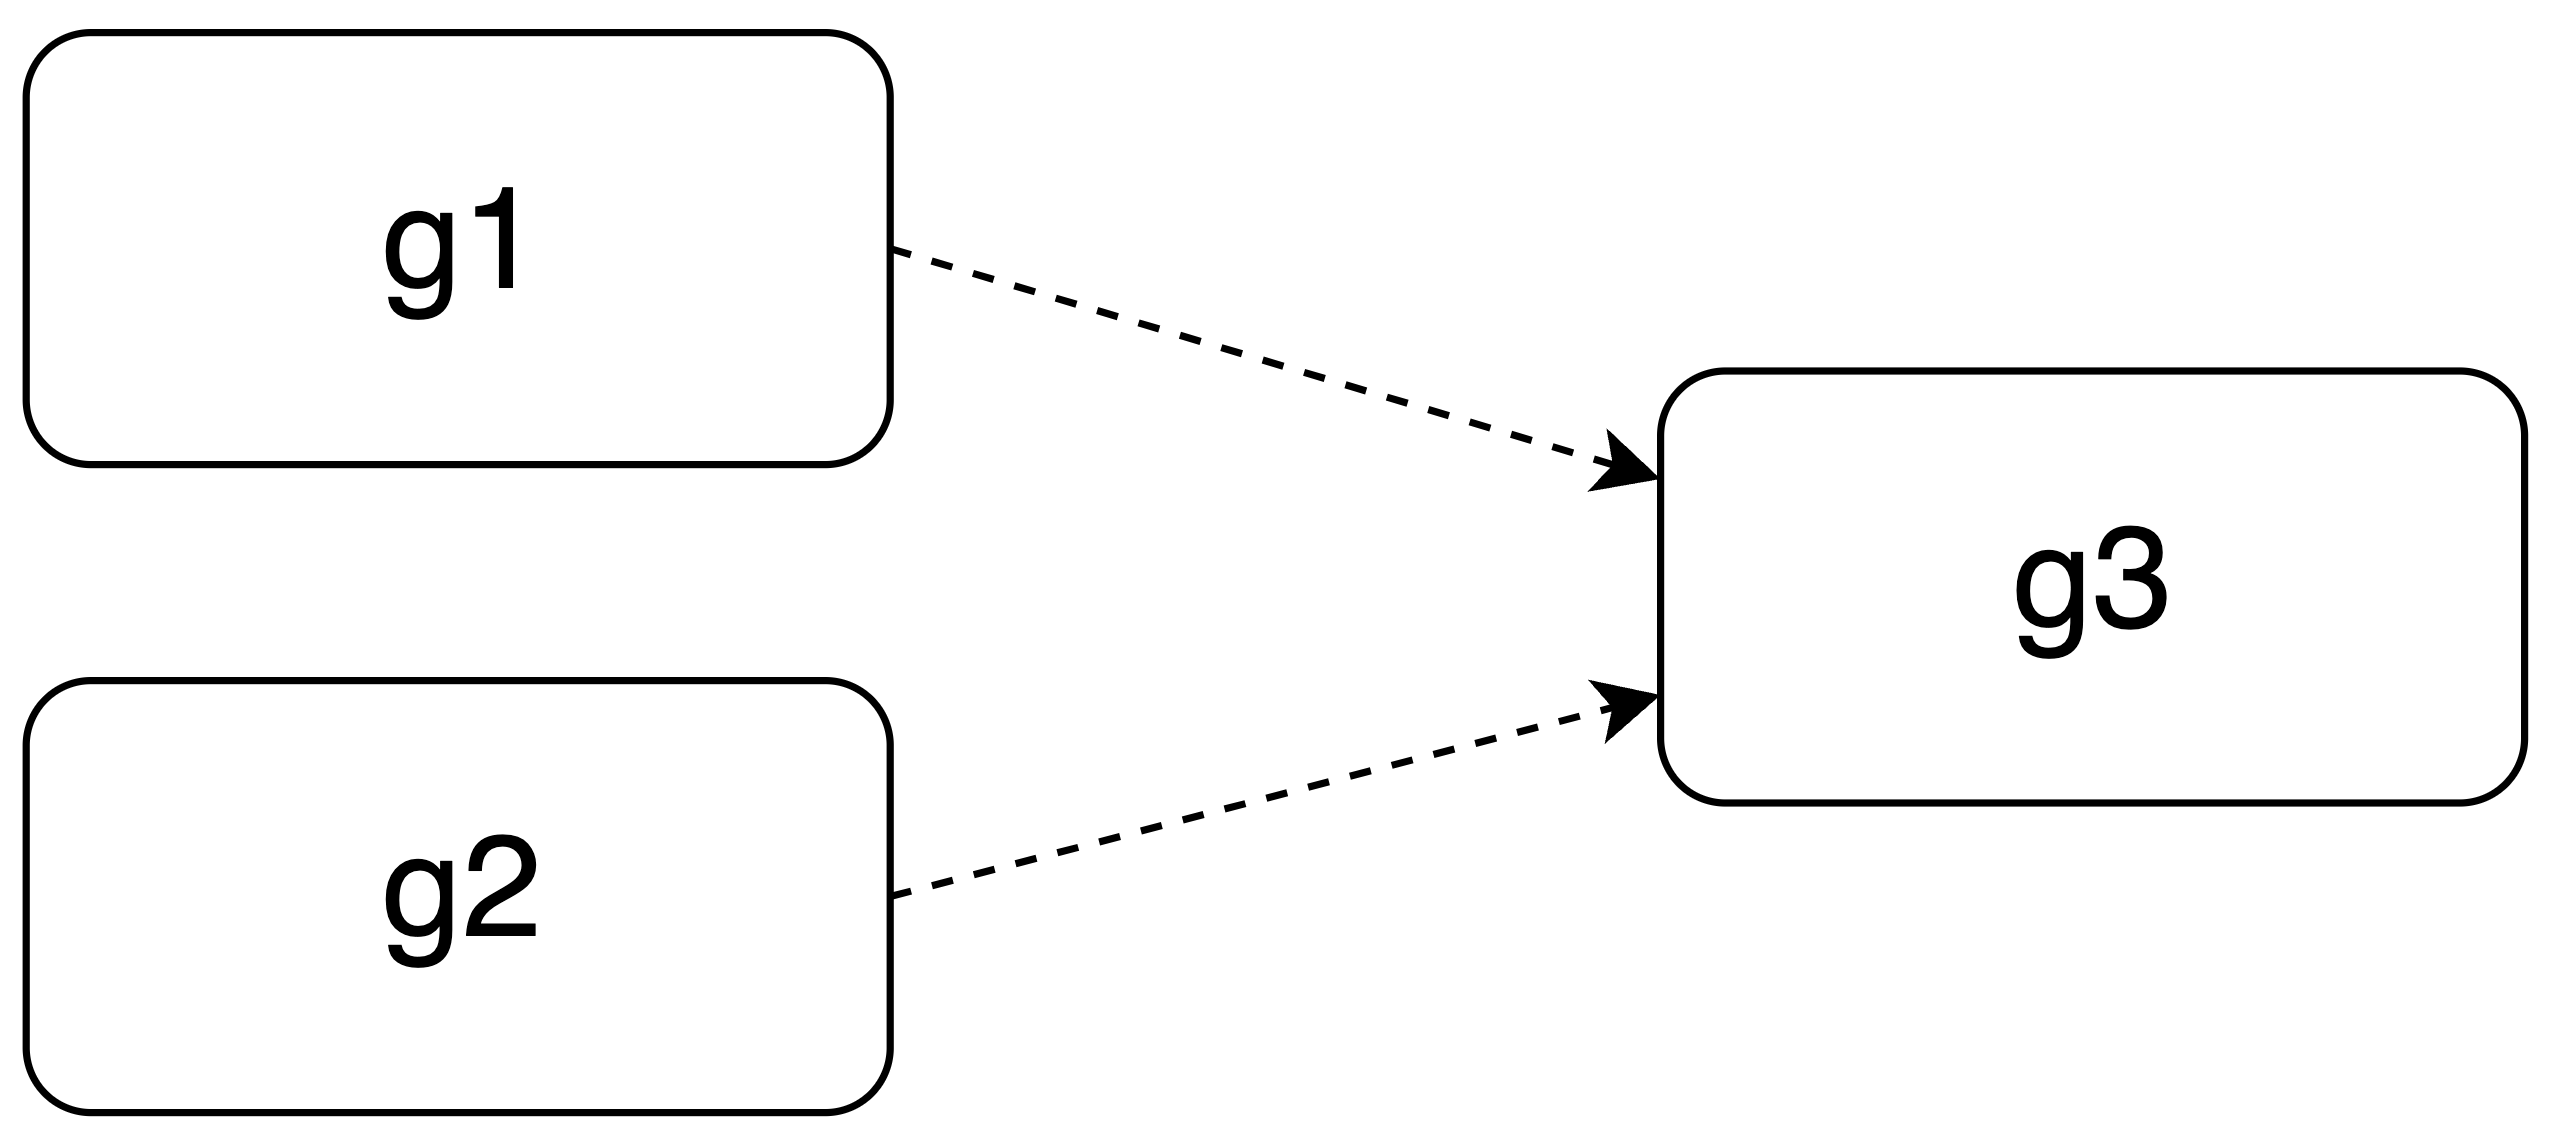
\includegraphics[width=0.7\textwidth]{images/visual-language/dependency-or.png}
        \end{figure}
    \end{column}
    \begin{column}{0.5\textwidth}
        \begin{figure}
            \centering
            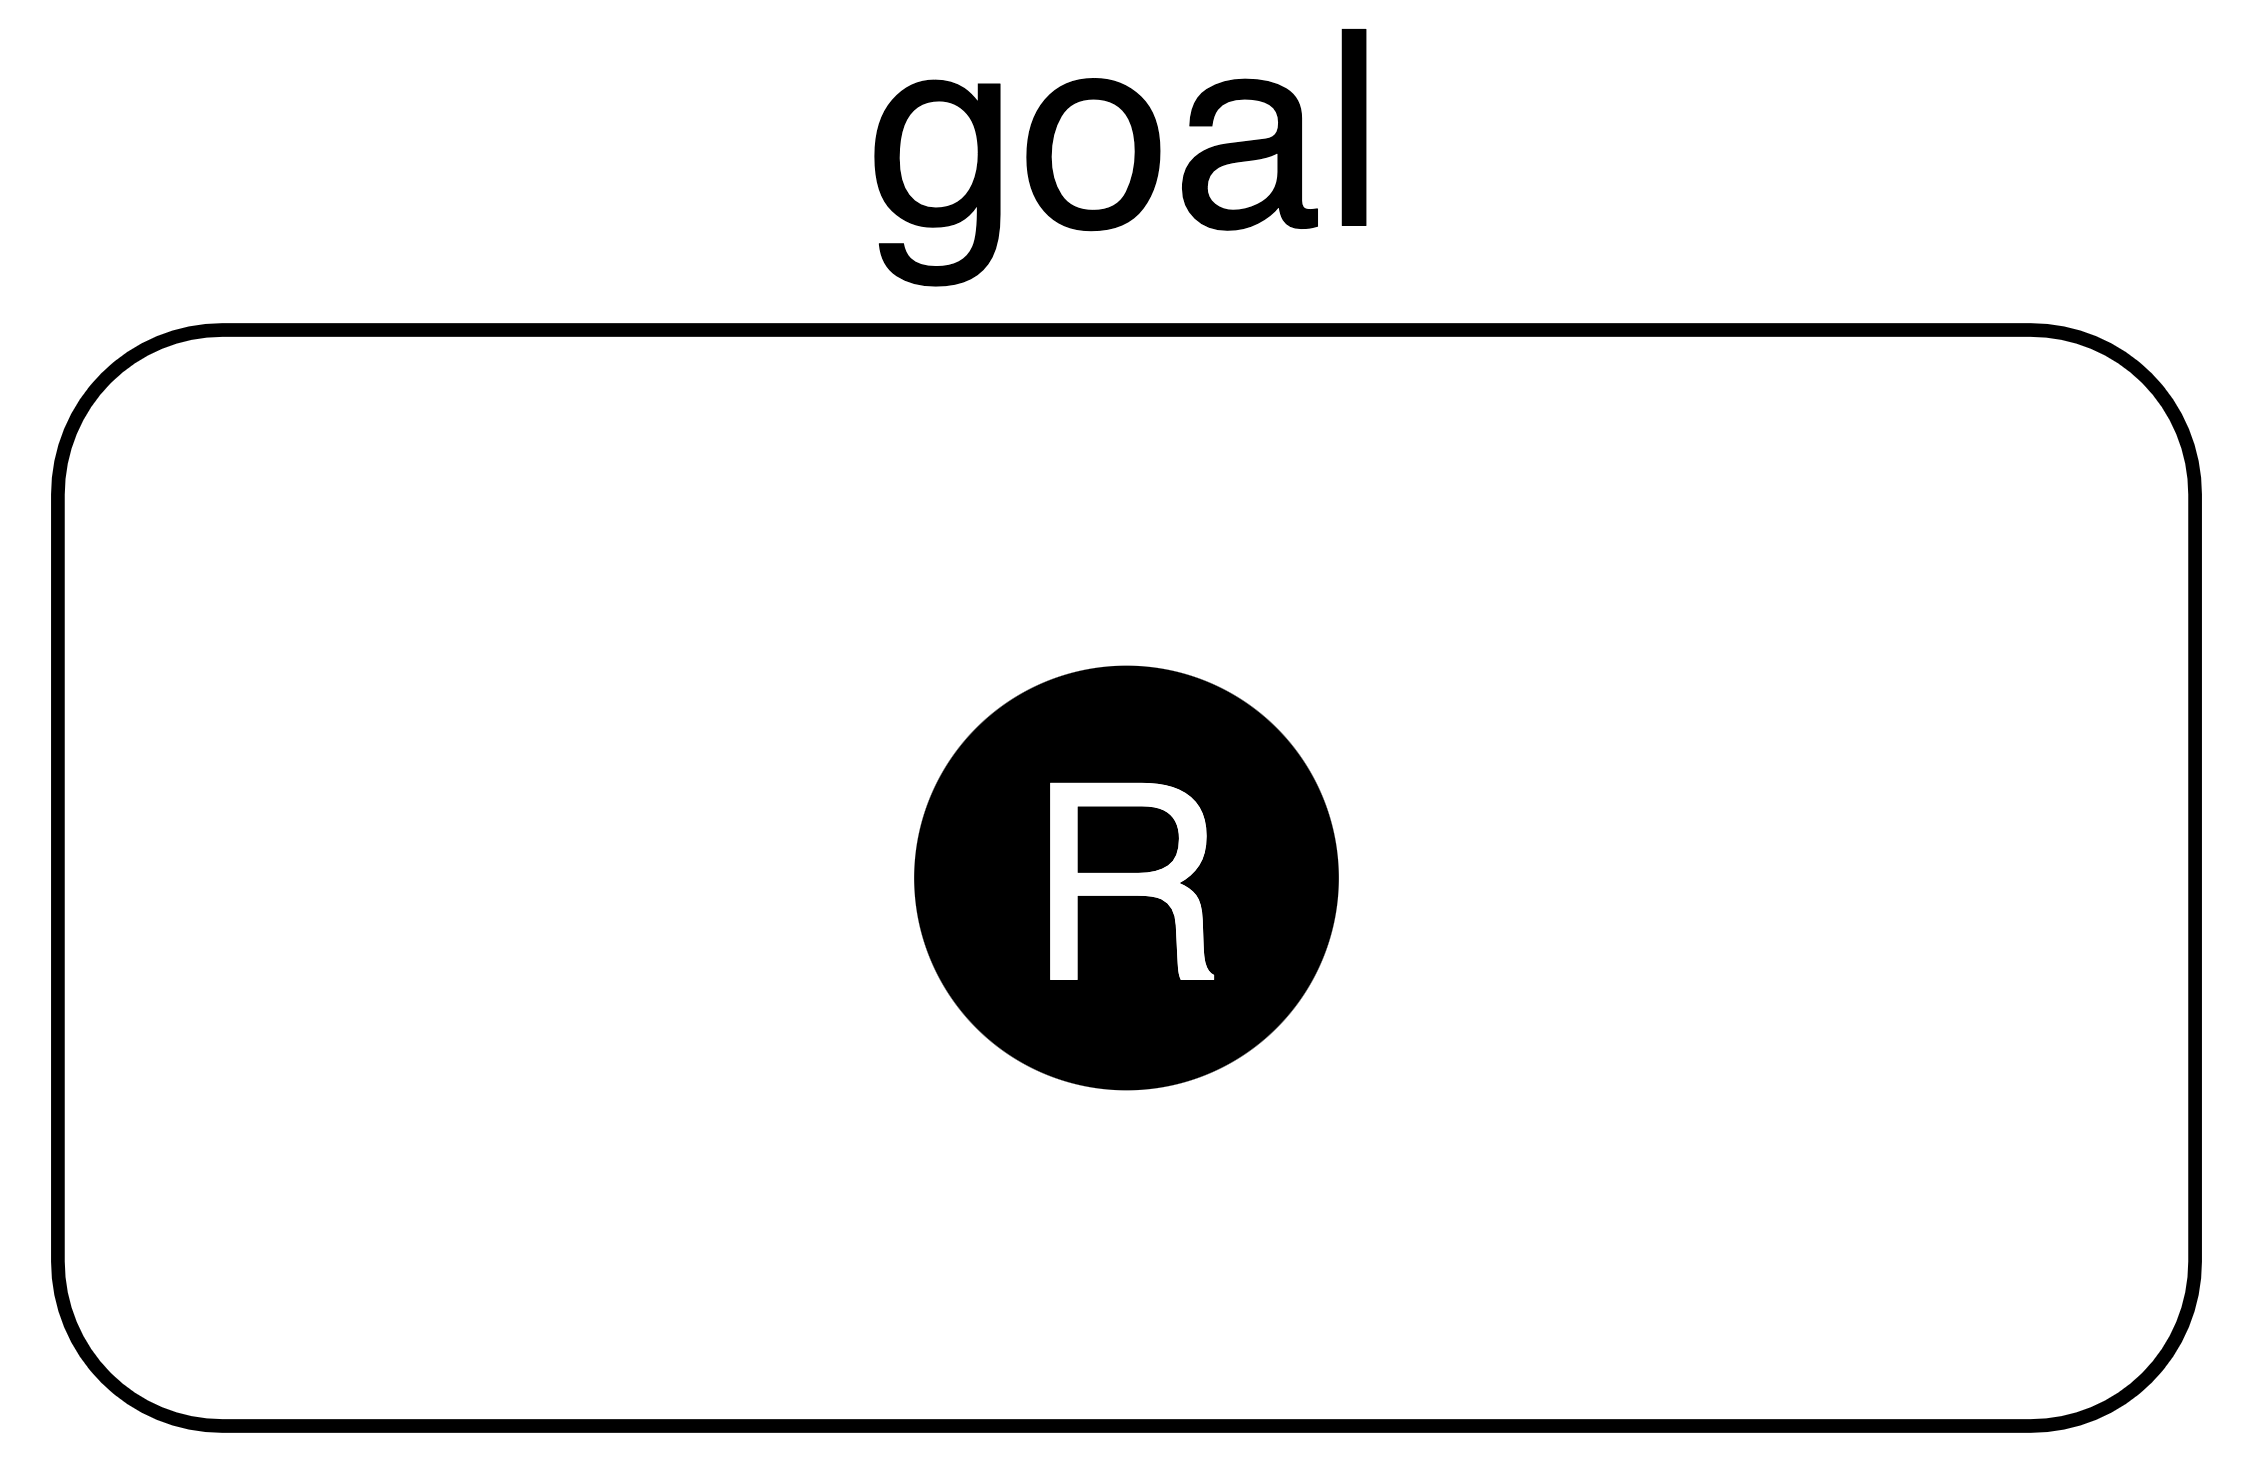
\includegraphics[width=0.35\textwidth]{images/visual-language/goal-allocation.png}
        \end{figure}
    \end{column}
\end{columns}

\end{frame}

\subsection{The Development Environment}
\begin{frame}[allowframebreaks]{The Development Environment}
    \hspace{-0.5cm}
    \begin{tikzpicture}
        \node (structural){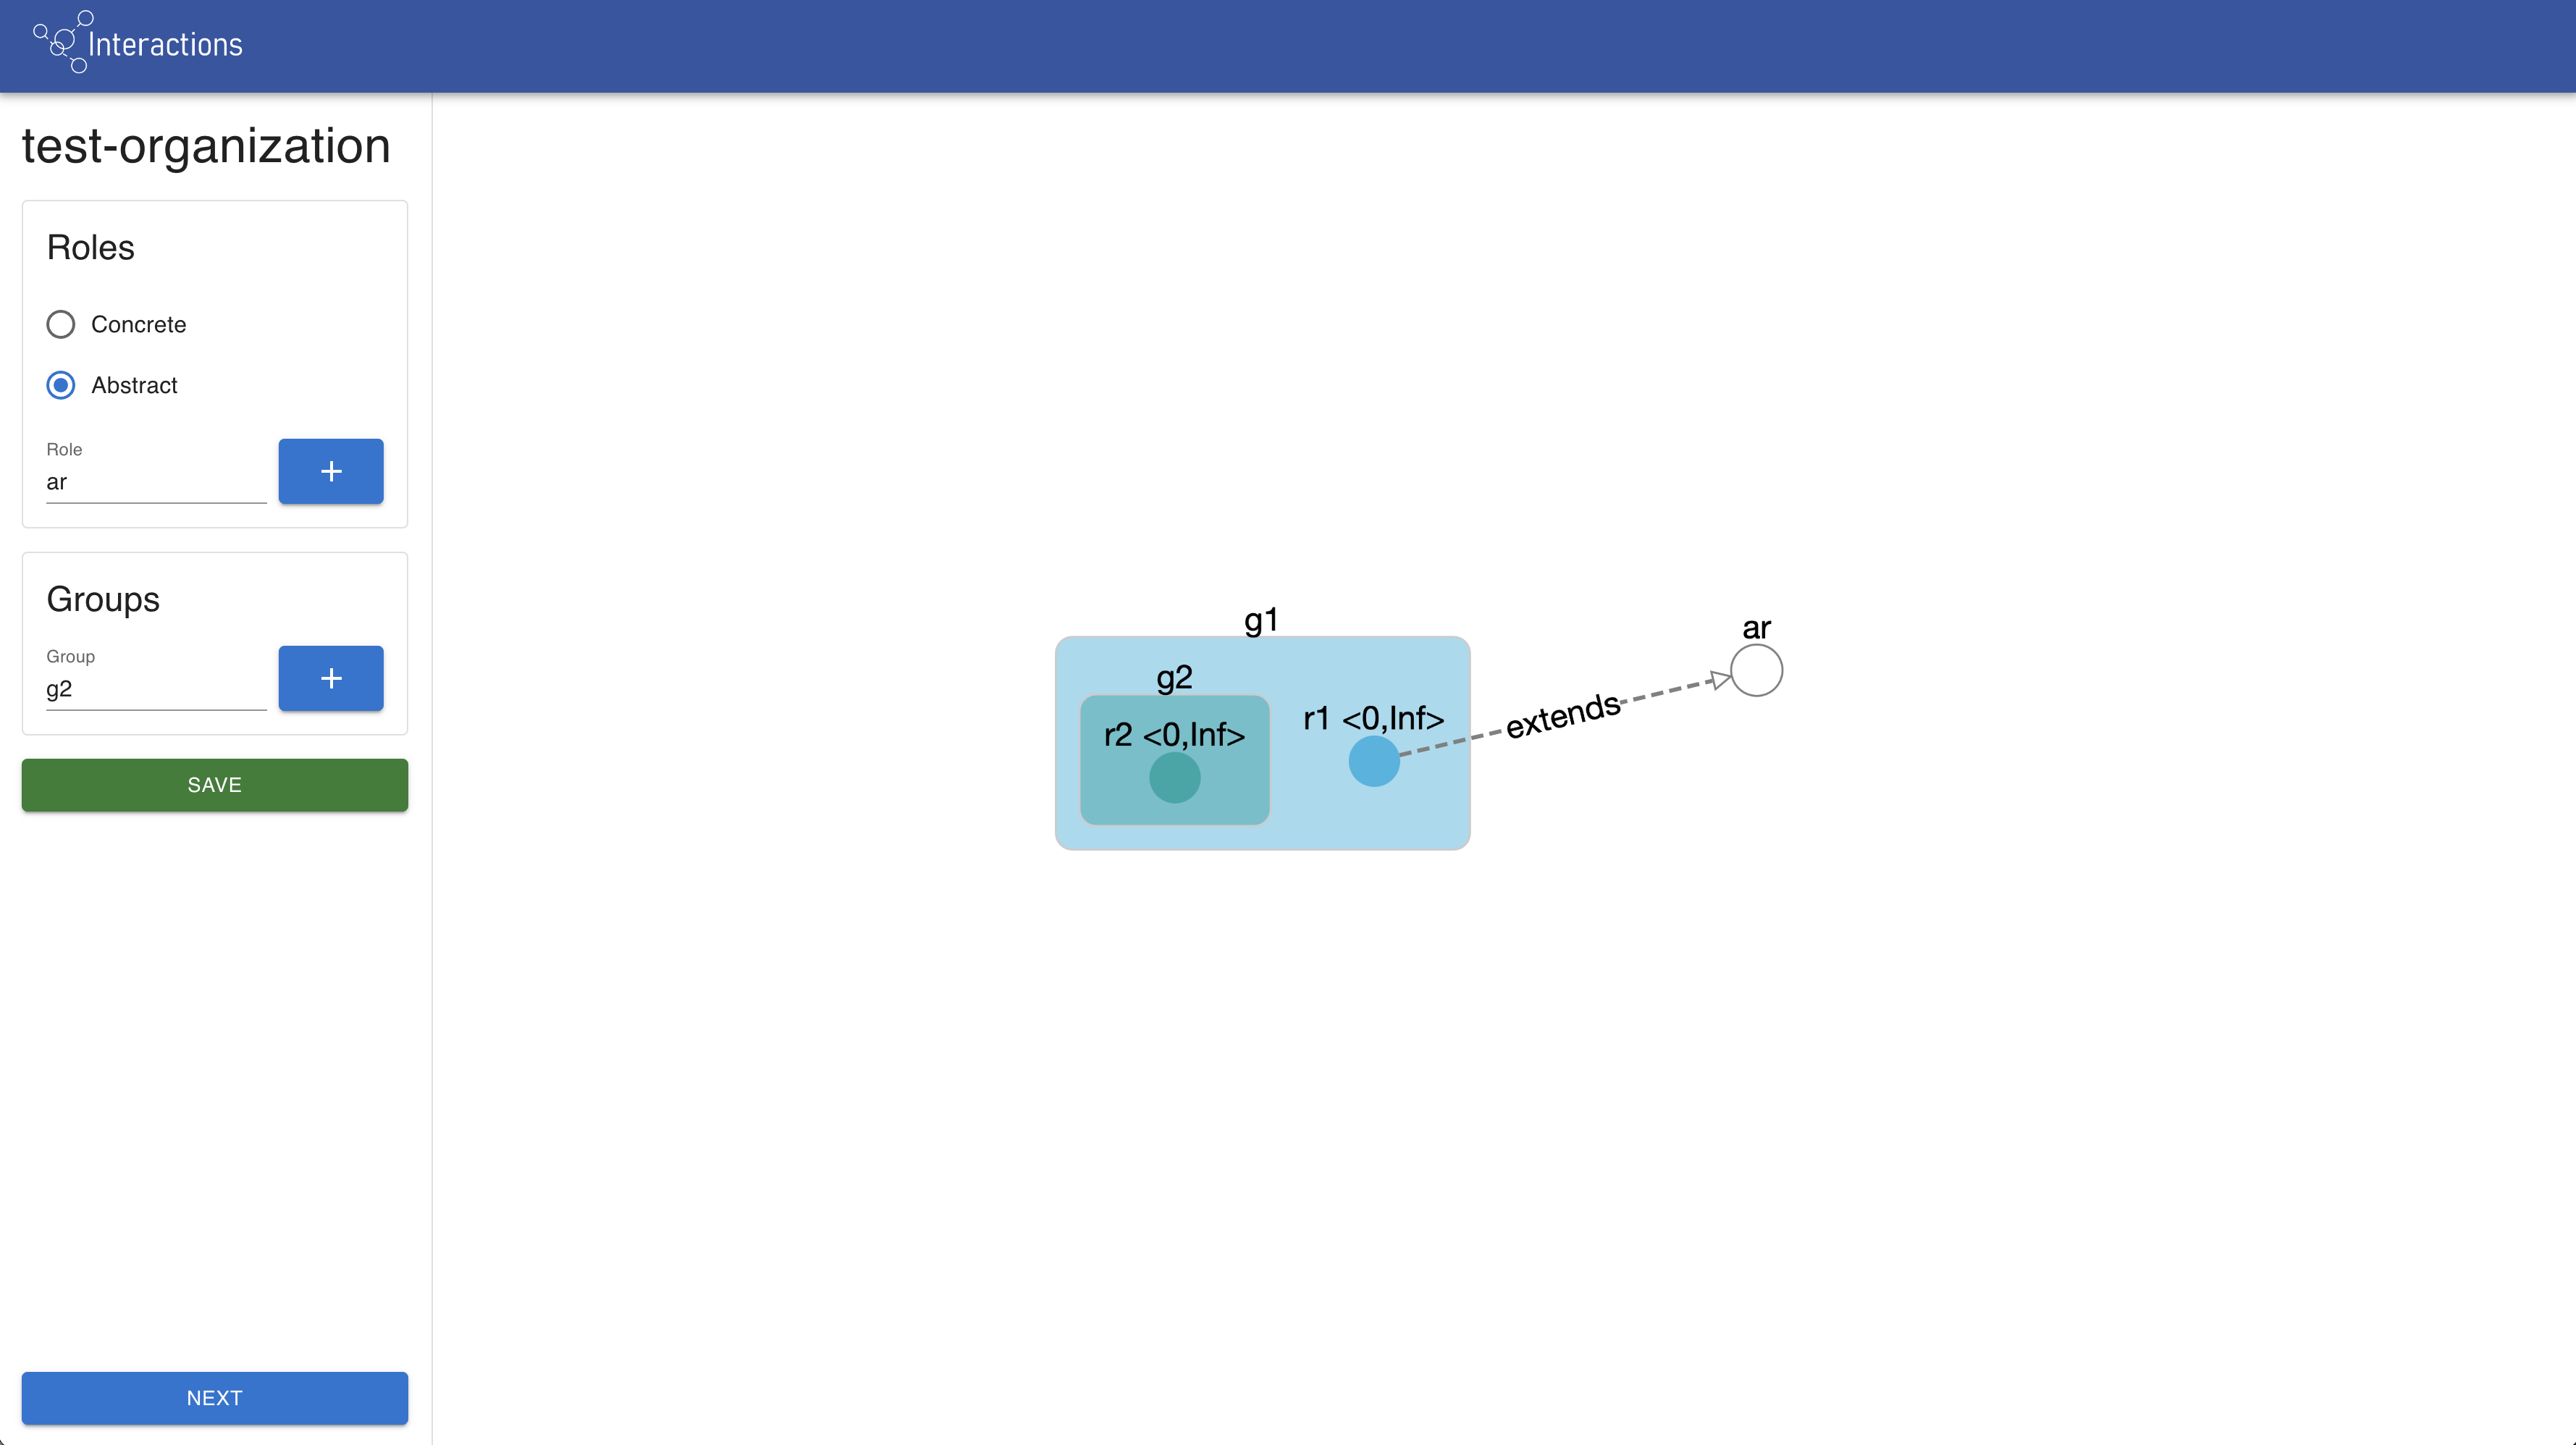
\includegraphics[height=4.2cm]{images/ide/structural.png}};
        \node (structural-side) at (structural.south east)[xshift=0.8cm,yshift=-0.5cm] {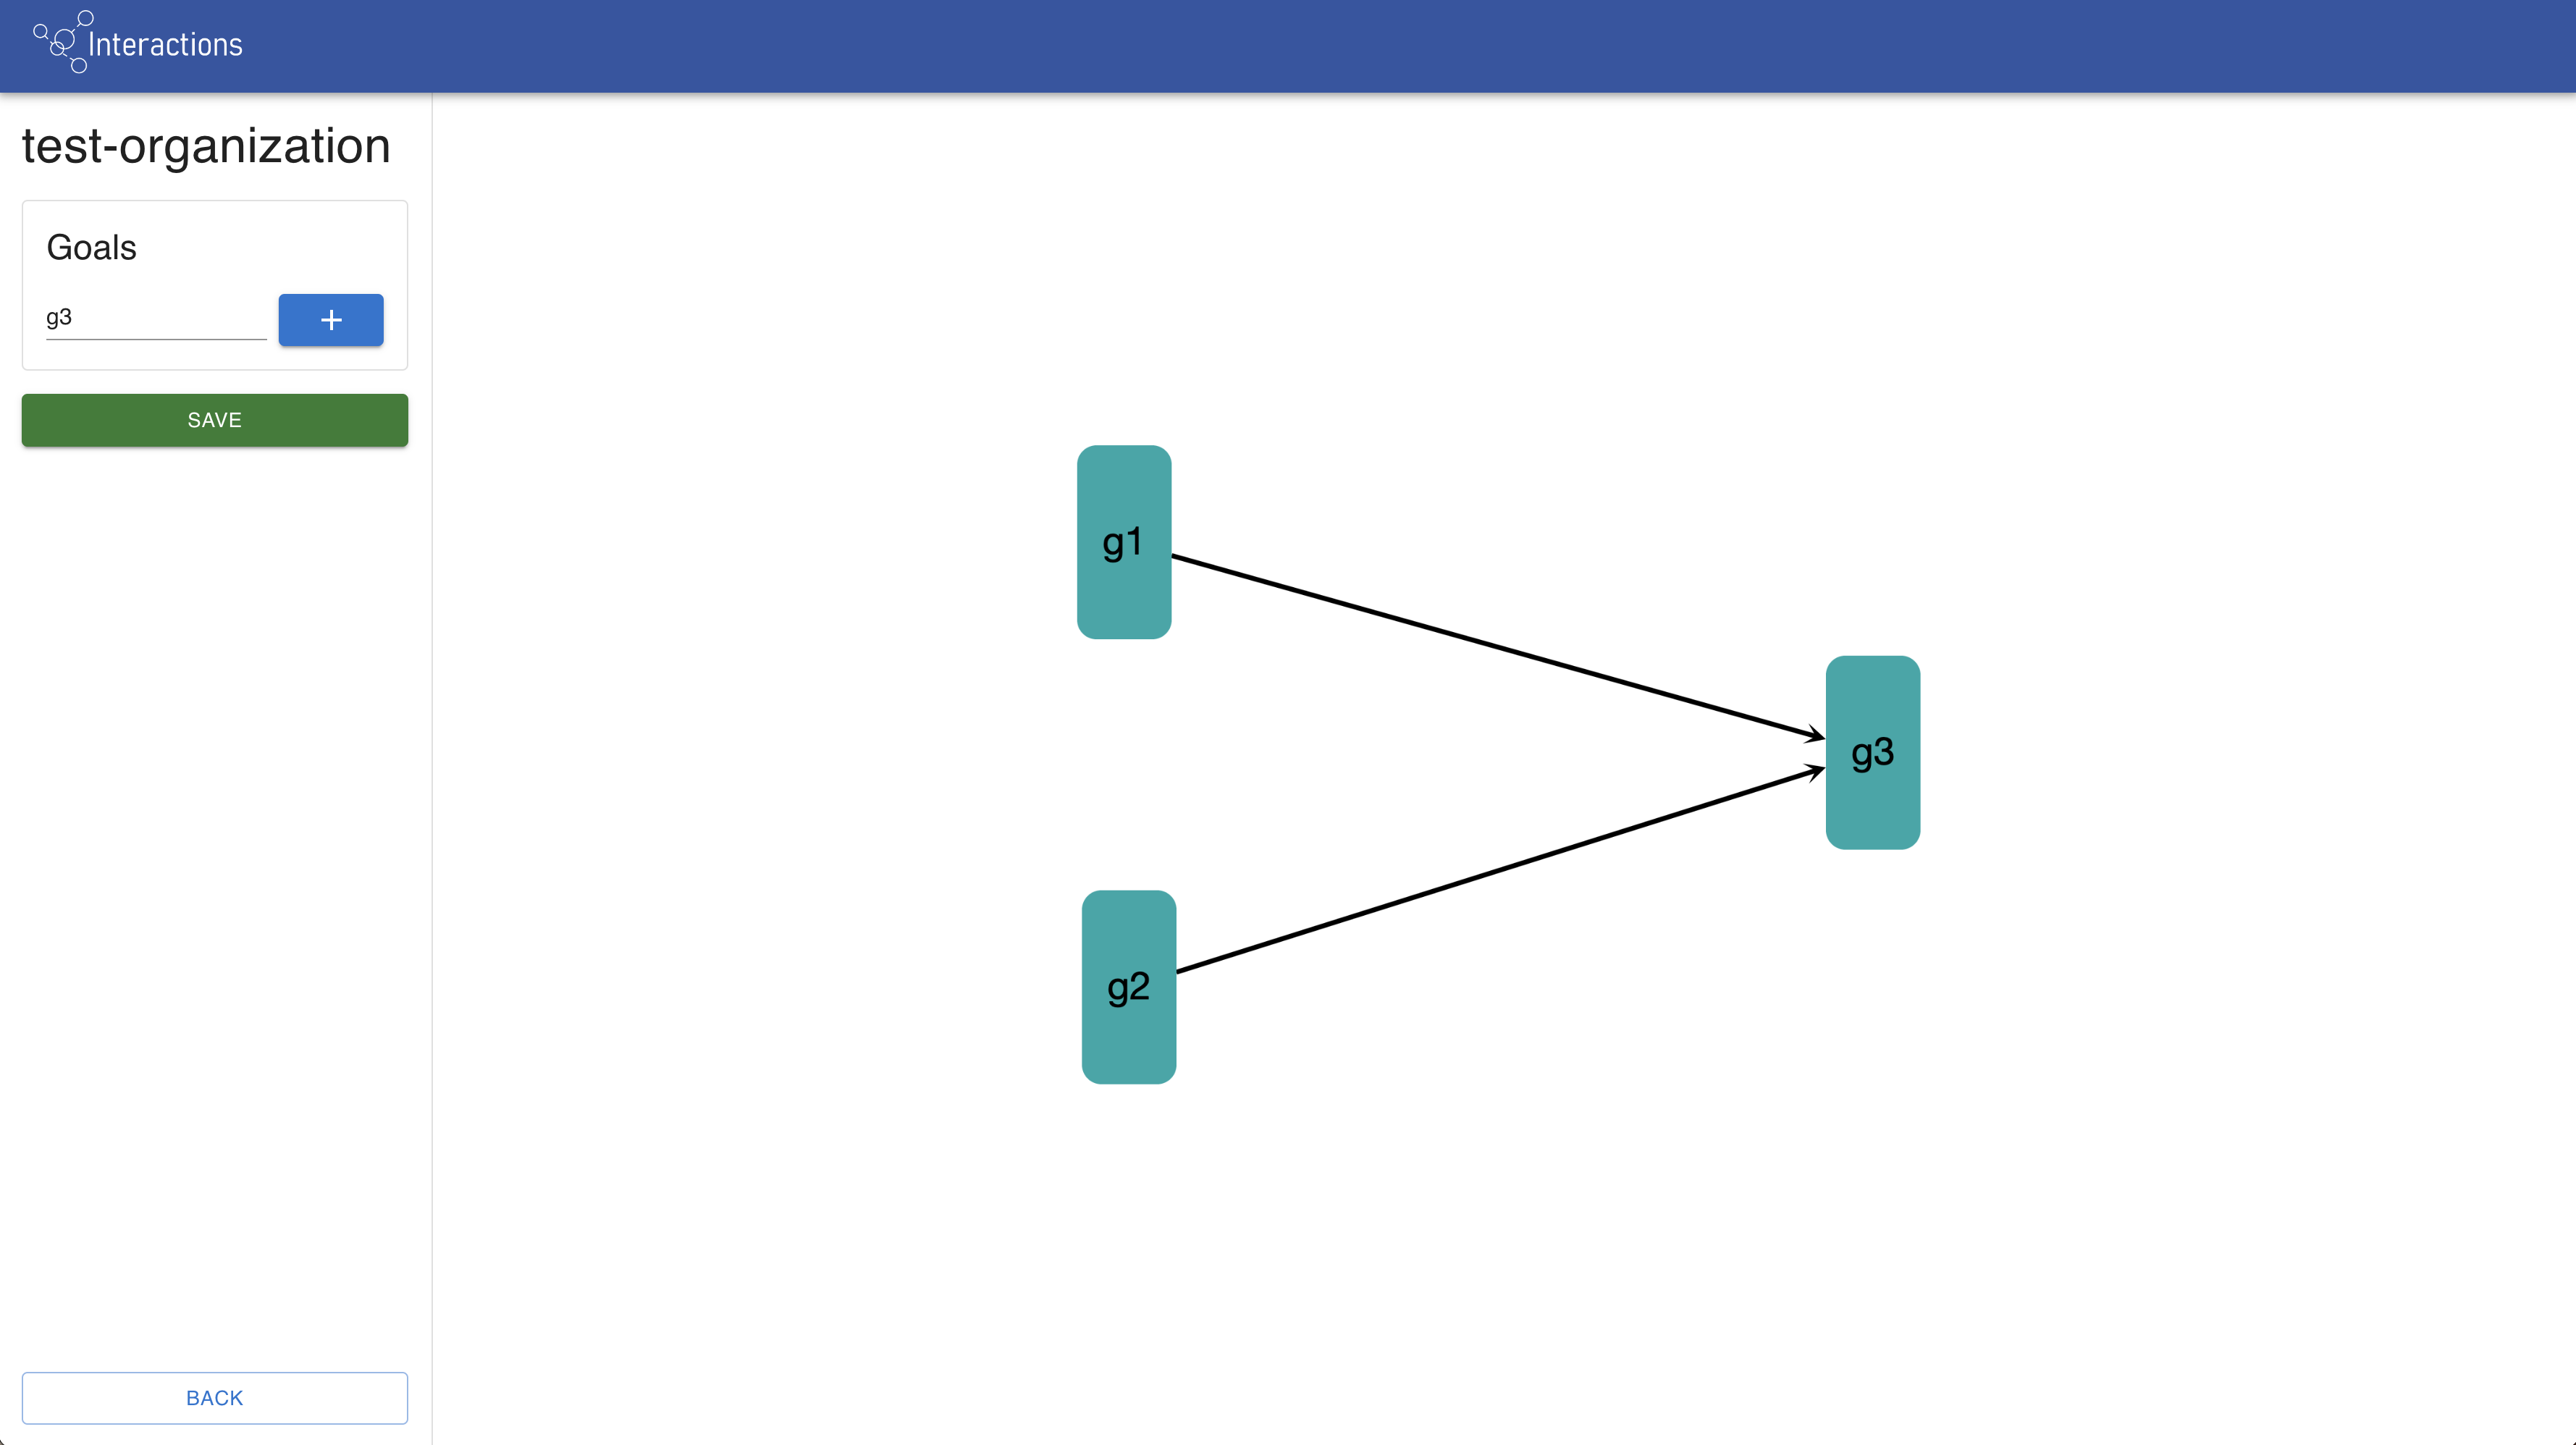
\includegraphics[height=4.2cm]{images/ide/functional.png}};
    \end{tikzpicture}

    \framebreak

    \begin{figure}
        \centering
        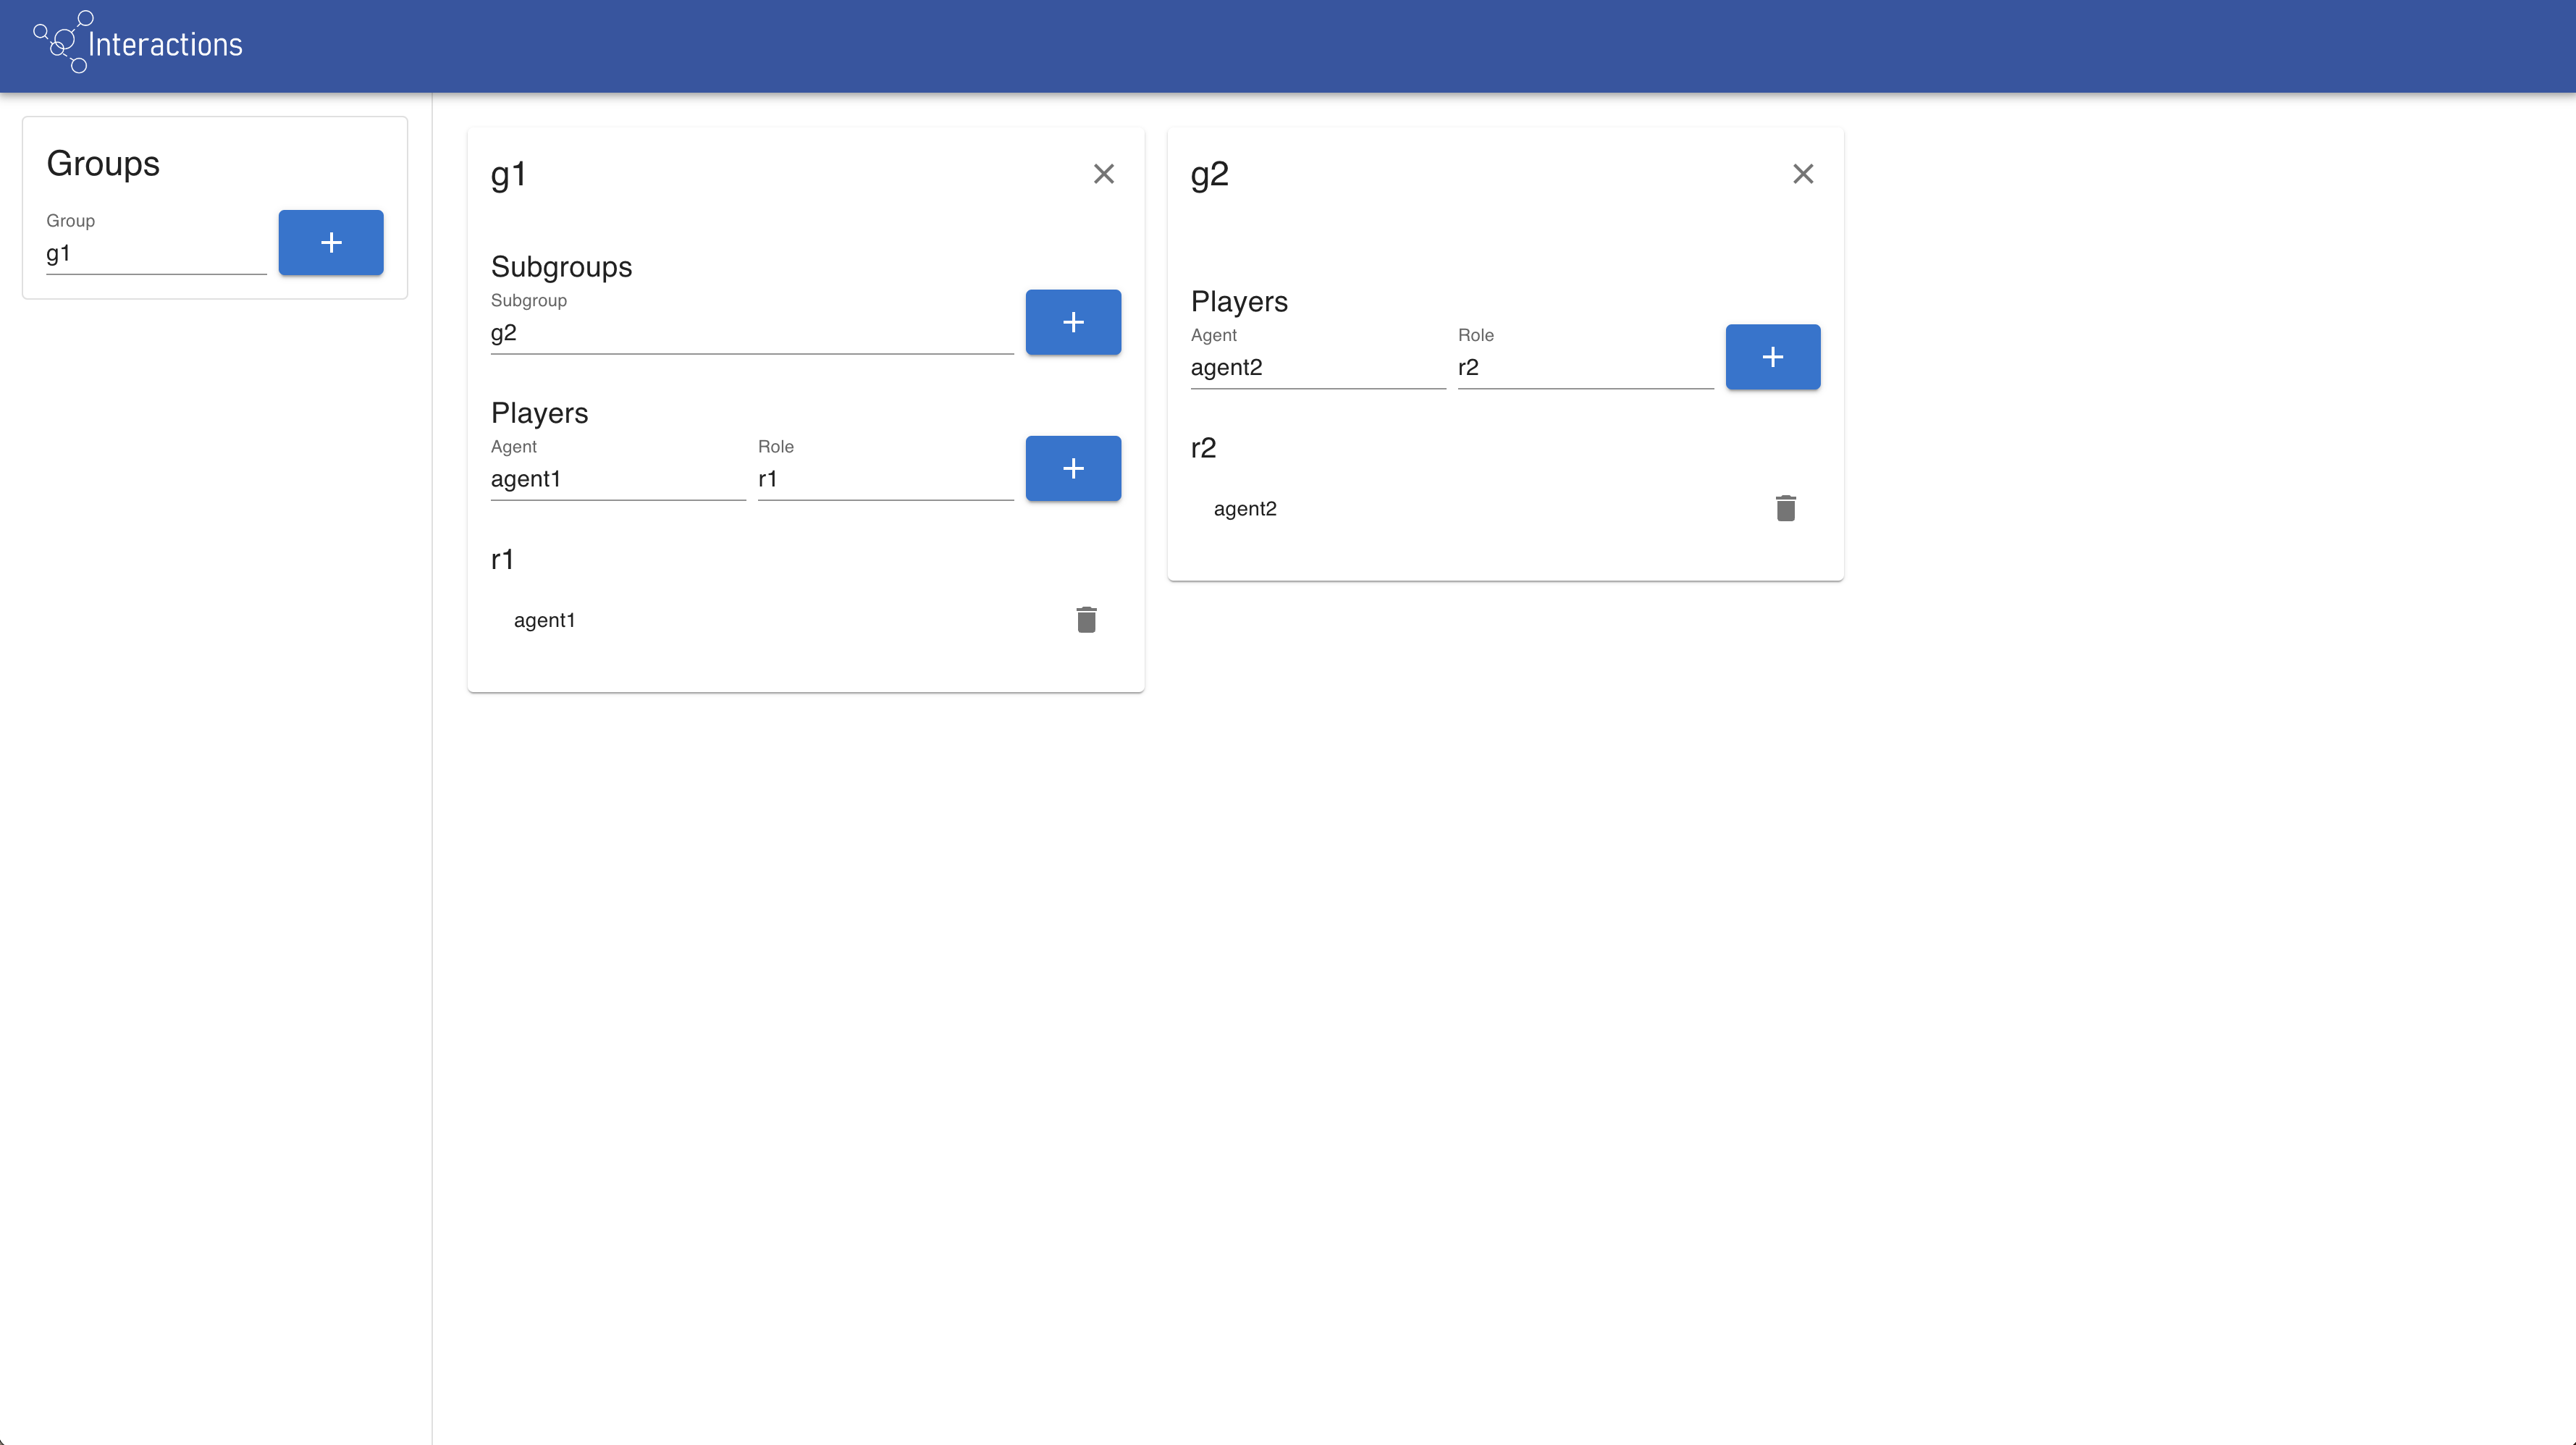
\includegraphics[width=\textwidth]{images/ide/entity.png}
    \end{figure}
\end{frame}

\subsection{Integration with the Runtime Environment}
\begin{frame}{Integration with the Runtime Environment}
    \begin{itemize}
        \item To deploy the created organizations, integration with the runtime environment is needed
        \item Domain experts can:
        \begin{itemize}
            \item Specify which groups will be deployed
            \item Access the agents running in the runtime environment
            \item Assign roles to agents
        \end{itemize}
        \item {Organizational artifacts}, which keep the information about the organization at runtime, are created
        \item Agents are told to join the organization and adopt the roles they were assigned
    \end{itemize}
\end{frame}